\begin{figure}
	\centering
		
	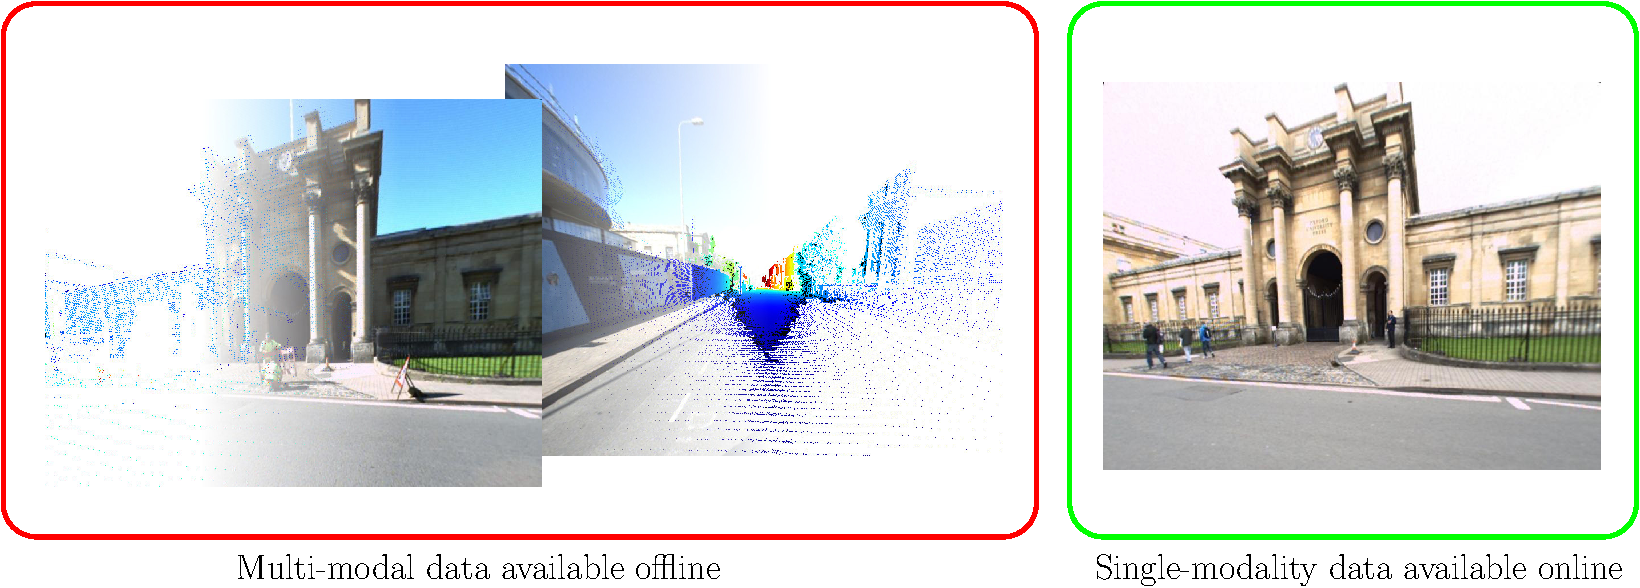
\includegraphics[width=\linewidth]{introduction/data_setup}

	\caption[Data partitioning]{\label{fig:data_setup} \textbf{Data partitioning within a practical localization scenario:} data available offline are richer than the one used during the localization task. We consider RGB (radiometric) + D (geometric) + R (material reflectance) as multi-modal data and only-RGB as single modality information.}
	
\end{figure}
	